\section{Packet Models}
\label{sec:packet_model}

Different messages are exchanged between nodes of the wireless networks.
Here are reported all the possible messages that a node could send or receive depending on its role in the network.

% Message beacon ---------------------------------------------------------------------------------
\subsection{Beacon message}

Beacon messages are used to built the tree topology of the network.

As shown in \cref{fig:msg_beacon}, every beacon contains:

% Items
\begin{itemize}

\item \textbf{seqn} The sequence number of the beacon periodically incremented by the sink.

\item \textbf{metric} And integer indicating the distance (hops) of the node which has sent the beacon from the sink.

\end{itemize}

% Figure
\begin{figure}[t]
	\centering
	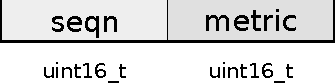
\includegraphics[width=0.5\columnwidth]{res/beacon}
	\caption{The beacon message contains two fields: \textit{seqn}  and \textit{metric}}.
	\label{fig:msg_beacon}
\end{figure}

The sink is the node that periodically broadcast beacon packets.
When a node  of the network receive a beacon, it analyzes the beacon's payload, its RSSI and decide if the packet is fresh enough to be take into consideration and to be retransmitted to other nodes. More details are described in the next section.


% Message data collection and command -------------------------------------------------------------

\subsection{Common messages}

The other messages that are exchanged between nodes, apart from beacons, have all the same structure and depending on the content of the header they have different meanings. 
The header is composed by two parts: the first has a fixed size while the second is an array of node addresses that, depending on its content, it have different lengths.

All the fields of packet are shown in \cref{fig:msg_packet} and described here:

\begin{itemize}

\item \textbf{source} Contains the address of the node which sent the packet.

\item \textbf{hops} Contains a counter incremented every time the packet is forwarded to another node.

\item \textbf{is\_command} A boolean flag that allows nodes to distinguish \texttt{command} packets typically sent by the sink from others messages.

\item \textbf{path\_length} Indicates the length of the array contained in bytes that immediately follow this field.

\item \textbf{path} All the bytes contained between the \texttt{path\_length} field and \texttt{data} are interpreded as an array of node's addresses. Depending on the type of packet, the array can be used by the sink to populate and update its routing table or it can contain the route that the packet should follow to reach its destination.

\item \textbf{data} The \texttt{data} part of the packet contains the payload read by the destination node.

\end{itemize}

% Figure
\begin{figure}[t]
	\centering
	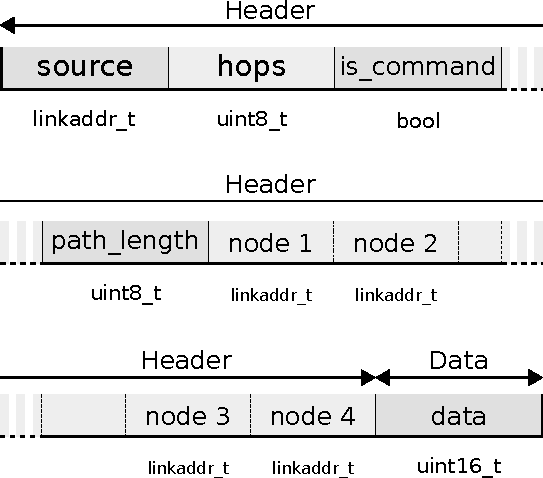
\includegraphics[width=0.8\columnwidth]{res/msg}
	\caption{Representation of a common packet exchanged by nodes. It is divided in header part and data part.}
	\label{fig:msg_packet}
\end{figure}

Here are described the different types of messages:

\begin{itemize}

\item \textbf{Data Collection Packets} This type of message is sent by any node that at certain time needs to report to the sink some data. The \textit{sender} node attaches to the message the data that has to send. In the header it specifies itself as the source, it initializes the hop field and insert its address in the array of node's addresses. 

Whenever one of the other nodes receives a message of this type, it tries to forward the packet to its parent until it reaches the sink. Before forwarding the packet, each node insert its address in the \texttt{path} array.

\item \textbf{Topology Report Packets} Topology Report packets are sent by every node to inform the sink about the current network topology. This kind of packets are similar to the Data Collection packets. They differs from the previous tipology only beacuse the \texttt{data} part of the packet is empty.

\item \textbf{Command Packets} These packets are used by the sink to send to a specific node in the network some data. The header's \texttt{path} field is filled with the route that the packet should follow to reach its destination. The \texttt{is\_command} flag is set to \textit{true} to inform the nodes to handle this packet differently from the other ones.

\end{itemize}



